\section{Planejamento Financeiro para Servidores}

\begin{frame}[c]\frametitle{Planejamento Financeiro}
  \textbf{Por que o planejamento financeiro se tornou essencial?}
  \begin{itemize}
    \item \textbf{Fim das Regras Antigas:} Aposentadoria não é mais igual ao último salário (fim da integralidade e paridade).
    \item \textbf{Benefício Limitado:} Proventos de aposentadoria de novos servidores são limitados ao teto do INSS.
    \item \textbf{Requisitos Mais Rigorosos:} A idade e o tempo de contribuição para se aposentar têm aumentado (exemplo: a idade mínima subiu 5 anos para homens na última grande reforma).
    \item \textbf{Insegurança Jurídica:} As regras da previdência têm mudado constantemente, tornando a projeção de longo prazo incerta.
  \end{itemize}
\end{frame}

\begin{frame}[t]\frametitle{Matéria do dia 17/08/2025 baseada numa pesquisa da FVG}

  \begin{center}
    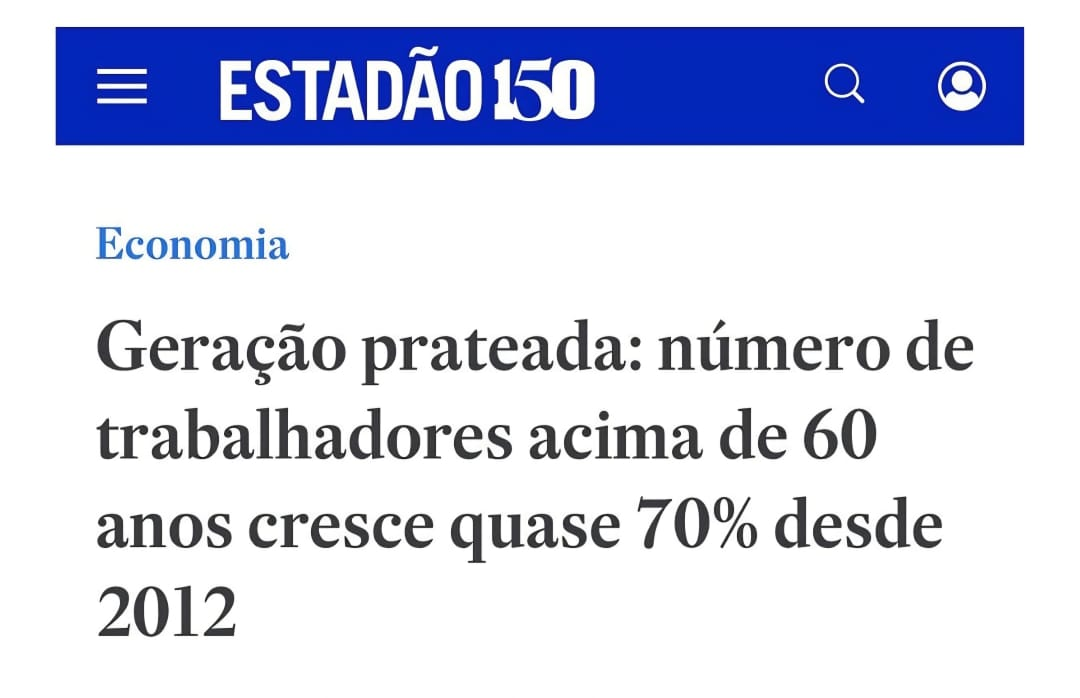
\includegraphics[width=0.8\textwidth]{figuras/geracao_prateada.jpeg}
  \end{center}

\end{frame}

\begin{frame}[c]\frametitle{Estratégias de Planejamento}
  \begin{itemize}
    \item \textbf{Projete sua Renda:} Calcule a diferença entre seu salário atual e o teto do INSS. Essa é a lacuna que seus investimentos precisam preencher.
    \item \textbf{Considere a Previdência Complementar (Funpresp):} Existe o benefício da paridade, onde o governo contribui com o mesmo valor que você.
    \item \textbf{Diversifique os Investimentos:} Não dependa apenas da Funpresp. Considere Tesouro Direto (proteção contra inflação) e outros investimentos.
    \item \textbf{Comece o Quanto Antes:} O tempo é seu maior aliado. Graças aos juros compostos, pequenos investimentos no início da carreira geram um grande patrimônio no futuro.
  \end{itemize}
\end{frame}